\section{Anforderungen Android und Device Management Server}
\label{sec:anforderungenandroiddevmgmt}

\subsection{Funktionsumfang bestehendes Aufnahmesystem}
Das bestehende TourLive System basiert auf einer Symbian App, die über Nokia Modelle (z.B. Nokia N82 und Nokia X6) betrieben werden. Die Daten (Positionsdaten, Bilder, Videostream) werden über das Mobilfunknetz via ein proprietäres Protokoll zum bestehenden TourLive-Server übertragen. Über eine Gerätestatusseite\footnote{bisherige Gerätestatusseite, \url{http://www.tourlive.ch/tds12/status.php}, aufgerufen am 27.02.2013}   können einfache Geräteverwaltungsaufgaben durchgeführt werden. Folgende Übersicht bietet einen groben Überblick über das aktuelle System: \url{
http://www.cnlab.ch/tourlive/Radrennen.html#TourLive_Aufnahmesysteme_im_Tour_Tross} \\

Das Symbian System soll nun auf Android portiert werden, wobei der Funktionsumfang für den ausschliesslichen Einsatz bei Radrennen eingegrenzt wird. 

\subsubsection{Views}
Die aktuelle Symbian App bietet folgende Views. Diese werden in 3 Spalten beschrieben, wobei die rechte Spalte einen Ausblick in die neue Android App und deren Funktionalität darstellt. Die Angaben unter „Neues System“ dienen jedoch nur der Übersicht und im Vergleich zum alten System. Eine exakte Spezifizierung inklusive neuer Funktionalitäten erfolgt im nächsten Kapitel.

Diese View wird beim Start der App angezeigt. Über die beiden Pfeile in der horizontalen Navigationsleiste wird über die verschiedenen Views navigiert.

\begin{longtable}{p{4.5cm} p{3cm} p{4.5cm}}
\textbf{Altes System - View GPS Info}
	\begin{itemize}	[noitemsep,nolistsep] 
		\item Geschwindigkeit [km/h]
		\item Höhe [m]
		\item Richtung (in Azimut) / Beschleunigung (Beschleunigung kann weggelassen werden)
		\item Steigung [\%]
		\item Latitude (Koordinate)
		\item Longitude (Koordinate)	 
	\end{itemize} 
	
	&   \raisebox{-\totalheight}{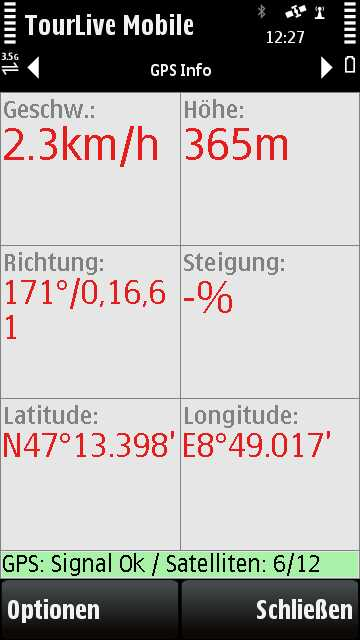
\includegraphics[width=3cm]{images/android/screensnap/GPSInfo.jpg}}
	& \textbf{Neues System} \newline
	\begin{itemize}		[noitemsep,nolistsep] 
		\item Geschwindigkeit [km/h]
		\item Höhe [m]
		\item Richtung (in Azimut) 
		\item Steigung [\%], über 100m gerechnet
		\item Latitude (Koordinate)
		\item Longitude (Koordinate)	
	\end{itemize}\\


	\textbf{Altes System - View Trip Info}  \newline
	View erreichbar durch einfaches Betätigen der „nach links“-Navigation.  	\begin{itemize}	[noitemsep,nolistsep] 
		\item Zeit Trip [hh:mm:ss]
		\item Höhe Trip [m]
		\item Distanz [km]
		\item Durchschnittliche Geschwindigkeit [km/h]
		\item UTC Zeit (Weltzeit)
		\item Datum (aktuelles Datum)
	\end{itemize}
	&   \raisebox{-\totalheight}{ 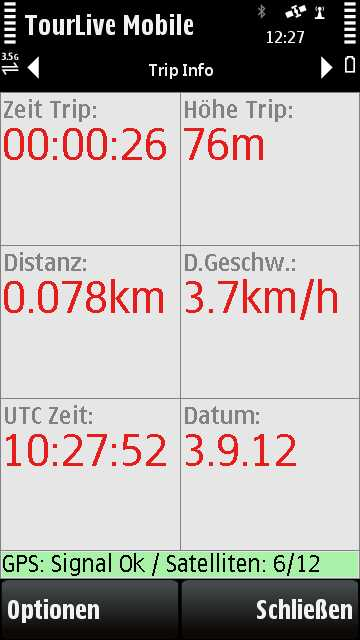
\includegraphics[width=3cm]{images/android/screensnap/TripInfo.jpg}  }
 	& \textbf{Neues System}\newline
	\begin{itemize}	[noitemsep,nolistsep]
		\item Zeit [hh:mm:ss]
		\item Höhe [m]
		\item Distanz [km]
		\item Durchschnittliche Geschwindigkeit [km/h]
	\end{itemize}\\

	\textbf{Altes System - View Total Info} \newline
	View erreichbar durch zweifaches Betätigen der „nach links“-Navigation.  
	\begin{itemize}[noitemsep,nolistsep]
		\item Zeit Total [hh:mm:ss]
		\item Zeit Tour [hh:mm:ss]
		\item Distanz Total [km]
		\item Distanz Tour [km]
		\item Höhe Total [m]
		\item Höhe Tour [m]
	\end{itemize} 
	&   \raisebox{-\totalheight}{ 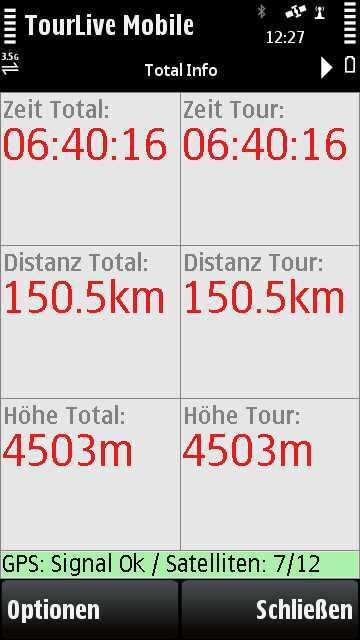
\includegraphics[width=3cm]{images/android/screensnap/TotalInfo.jpg}  }
	& \textbf{Neues System} \newline
	Diese View fällt weg. Es werden nur noch Daten pro Etappe erfasst. \\
	

	\textbf{Altes System -  View ODB Info} \newline 
	View erreichbar durch einfaches Betätigen der „nach rechts“-Navigation.    \newline
On Board Diagnose Bus (war für Benzinverbrauch, Motordrehzahl)	Bezieht sich auf ein externes Gerät. Ist im neuen System irrelevant und wird deshalb an dieser Stelle nicht dokumentiert. \newline 
	& \newline \newline Bezieht sich auf ein externes Gerät. Ist im neuen System irrelevant und wird deshalb an dieser Stelle nicht dokumentiert.  
	&\textbf{Neues System} \newline \newline 
Diese View fällt weg. Ein OBD wird nicht mehr benötigt. \\
	
	\textbf{Altes System -   View ODB Verbrauch} \newline 
	iew erreichbar durch zweifaches Betätigen der „nach links“-Navigation. 
	& \newline \newline Bezieht sich auf ein externes Gerät. Ist im neuen System irrelevant und wird deshalb an dieser Stelle nicht dokumentiert. \newline
	&\textbf{Neues System} \newline \newline 
Diese View fällt weg. \\
	
	\textbf{Altes System -  View Puls Info} \newline  
	View erreichbar durch dreifaches Betätigen der „nach links“-Navigation. \newline
On Board Diagnose Bus (war für Benzinverbrauch, Motordrehzahl)	Bezieht sich auf ein externes Gerät. Ist im neuen System irrelevant und wird deshalb an dieser Stelle nicht dokumentiert. \newline 
	& \newline \newline Bezieht sich auf ein externes Gerät. Ist im neuen System irrelevant und wird deshalb an dieser Stelle nicht dokumentiert.  
	&\textbf{Neues System} \newline \newline 
Diese View fällt weg. Ein OBD wird nicht mehr benötigt.\\
	
	\textbf{Altes System -   View ODB Verbrauch} \newline 
	iew erreichbar durch zweifaches Betätigen der „nach links“-Navigation. 
	& \newline \newline Bezieht sich auf ein externes Gerät. Ist im neuen System irrelevant und wird deshalb an dieser Stelle nicht dokumentiert.
	&\textbf{Neues System} \newline \newline 
Diese View fällt weg. Ein externes Puls Messgerät wird nicht mehr benötigt.\\


	\textbf{Altes System - View Netz Info}  \newline
	View erreichbar durch vierfaches Betätigen der „nach links“-Navigation.  
	\begin{itemize}[noitemsep,nolistsep]
		\item Zellen ID (Funkzellen Nummer)
		\item Area (Location Area)
		\item Signal (Signalstärke in dB)
		\item Akku (Akku Ladestatus)
		\item Netzwerk (Provider) 
		\item Netzwerk ID (Verbindungseigenschaften) \newline
		228 = Mobile Network Code \newline
		01 = Mobile Country Code \newline
		UMTS = Technologie
	\end{itemize}
	&   \raisebox{-\totalheight}{ 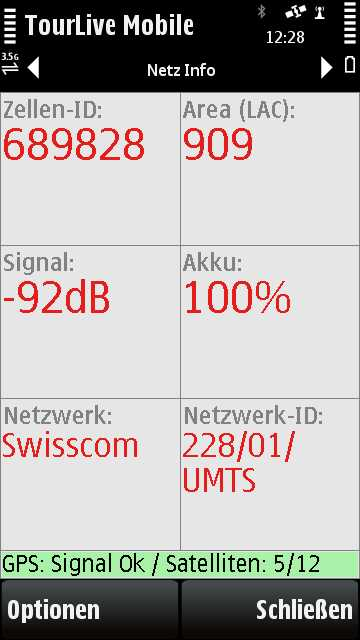
\includegraphics[width=3cm]{images/android/screensnap/NetzInfo.jpg}  }
 	& \textbf{Neues System} 
	\begin{itemize}	[noitemsep,nolistsep]
		\item Zellen ID
		\item Area
		\item Signal
		\item Netzwerk ID
		\item Technologie (UMTS) 
		\item Datenrate \newline
	\end{itemize}
		\textbf{Zusätzlich}
	\begin{itemize}	[noitemsep,nolistsep]
		\item RTT
		\item Packet-Loss
	\end{itemize}\\


	\textbf{Altes System - View Logs}  \newline
View erreichbar durch fünffaches Betätigen der „nach links“-Navigation.   \newline
Log um Fehlerquellen zu eruieren. \newline

	&   \raisebox{-\totalheight}{ 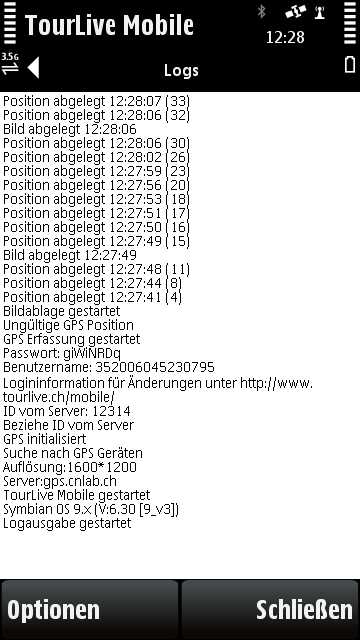
\includegraphics[width=3cm]{images/android/screensnap/Logs.jpg}  }
 	& \textbf{Neues System} \newline 
	Diese View wird in einem ähnlichen Stil beibehalten.\\


	\textbf{Altes System - View Hauptmenü}  \newline
	View wird sichtbar durch das Betätigen des „Optionen“-Buttons.
	\begin{itemize}[noitemsep,nolistsep]
		\item Start der Aufzeichnung
		\item Konfiguration der App (siehe unten)
		\item Bild auslösen (manuelle Bildauslösung)
		\item Hintergrundbe- leuchtung (Ein / Ausschalten > Stromsparfunktion)
		\item ODB > nicht mehr relevant
		\item Puls > nicht mehr Relevant
		\item GPS [Submenü]
		\item Reset GPS Trip Daten
		\item Reset GPS Tour Daten
		\item Reset alle GPS Daten
	\end{itemize}
	&   \raisebox{-\totalheight}{ 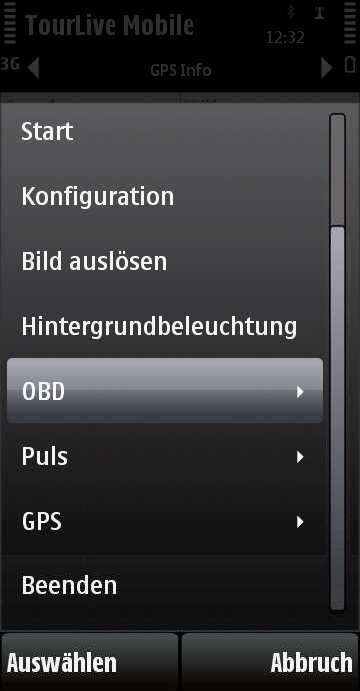
\includegraphics[width=3cm]{images/android/screensnap/Hauptmenue_1.jpg}  }
 	& \textbf{Neues System} \newline
	\begin{itemize}[noitemsep,nolistsep] 
		\item Einstellungen
		\item About
	\end{itemize}\\


	\textbf{Altes System - View Konfiguration}  \newline
	View wird sichtbar durch das Betätigen des „Konfiguration“-Buttons im Optionen-Menü.
	\begin{itemize}[noitemsep,nolistsep]
		\item Benutzername
		\item Grösse (irrelevant in der neuen Version)
		\item Gewicht (irrelevant in der neuen Version)
		\item Alter (irrelevant in der neuen Version)
		\item Geschlecht (irrelevant in der neuen Version)
		\item GPS Intervall (0 – 600 sec)
		\item GPS Speichern Intervall (0 – 600 sec)
		
	\end{itemize}
	&   \raisebox{-\totalheight}{ 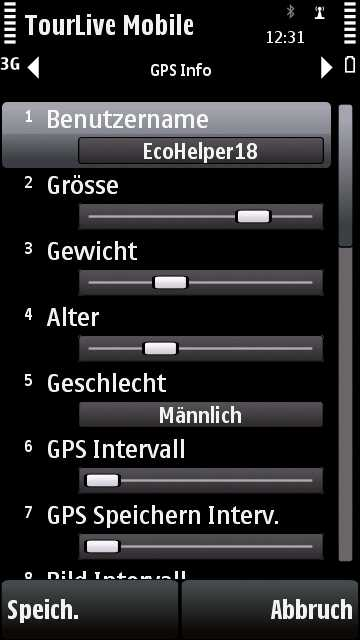
\includegraphics[width=3cm]{images/android/screensnap/Konfiguration_1.jpg}  }
 	& \textbf{Neues System} \newline
	\begin{itemize}	[noitemsep,nolistsep]
		\item Benutzername
		\item GPS Intervall (0 – 60 sec)
		\item GPS Speichern Intervall (0 – 600 sec) (Wird mit GPS Intervall zusammengefasst)
		\item Bild Intervall (0 – 60 sec)
		
	\end{itemize}
	\\

	\begin{itemize}[noitemsep,nolistsep]
		\item Bild Intervall  (0 – 600 sec)
		\item Einheiten (km – Meilen - ..) (nur noch MKS Einheiten standardmässig)
		\item Zusatzgerät (irrelevant in der neuen Version)
		\item Video Streaming (Ein / Aus)
		\item Bilder drehen (Ein / Aus)
		\item Offline Mode (Ein / Aus) (irrelevant in der neuen Version, wird automatisch gemacht)
		\item GPS Dateiformat (TourLive + Google Earth, Google Earth) (irrelevant in der neuen Version, wird serverseitig gerechnet)
	\end{itemize}
	&  \raisebox{-\totalheight}{ 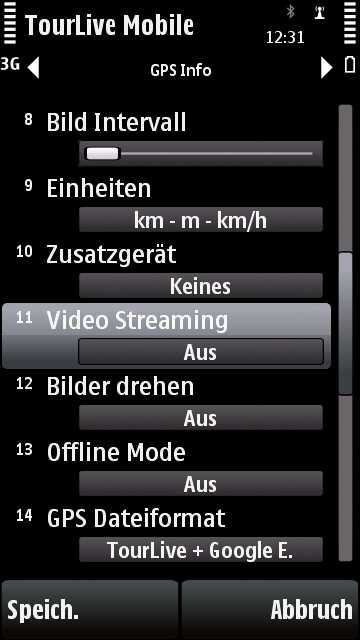
\includegraphics[width=3cm]{images/android/screensnap/Konfiguration_2.jpg}  } 
 	& 
	\begin{itemize}	[noitemsep,nolistsep]
		\item Bild Intervall (0 – 60 sec)
		\item Video Streaming (Ein / Aus)
		\item Bilder drehen (Ein / Aus)
		\item Automatischer Start (Neu verschiedene Modi)
		\item Hintergrundbeleuchtung (Normal / Dauernd an)
		\item Bildauflösung
		\item Bildmodus
	\end{itemize}\\

\begin{itemize}[noitemsep,nolistsep]
\item Automatischer Start (Ein / Aus)
\item Hintergrundbe- leuchtung (Normal / Dauernd an)
\item Einfaches Beenden (Ein / Aus) (irrelevant in der neuen Version)
\item Schreibe Logfile (Ein / Aus) (irrelevant in der neuen Version, wird immer geschrieben)
\item Heartbeat Ton (Lautstärke) (irrelevant in der neuen Version, keine Töne mehr)
\item Fehlerton (Lautstärke) (irrelevant in der neuen Version, keine Töne mehr)
\item Bildauflösung (1600 x 1200 , …)
\item Bildmodus (Portrait / Landscape)

\end{itemize}
	&  \raisebox{-\totalheight}{ 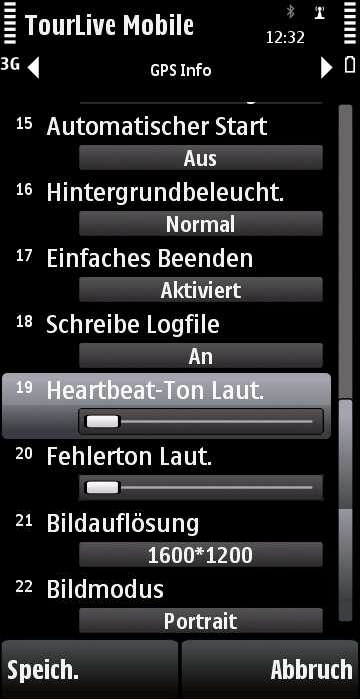
\includegraphics[width=3cm]{images/android/screensnap/Konfiguration_3and4_combined.jpg}  } 
 	& 
	\textbf{Zusätzlich} 
	 \begin{itemize}[noitemsep,nolistsep]
		\item Kritischer Akkustand
		\item Betriebsmodus
		\item TourLive Server Primär
		\item TourLive Server Sekundär
		\item Device Management Server
		\item Kamera automatisch ausrichten
		\item Videoauflösung
		\item Renndistanz Korrektur
		\item Gespeicherte Daten löschen
	\end{itemize}\\

\end{longtable}
 


\subsection{Anforderungen – Neues Aufnahmesystem}
Das neu zu entwickelnde Aufnahmesystem basiert grundsätzlich auf der Funktionalität der  bestehenden Symbian App. Wobei auf die Unterstützung  externer Geräte (Puls-Messung, Onboard Diagnose Bus (OBD)), verzichtet werden kann. Einen Überblick über die übernommenen Funktionen bietet die dreispaltige Beschreibung im Kapitel „Funktionsumfang bestehendes Aufnahmesystem [Symbian App]“.

\subsubsection{Hardware / Software - Aufnahmesystem}
Bei den Aufnahmegeräten wird gemäss Vorgabe des Auftraggebers auf das Betriebssystem Android ab Version 4.x (Ice Cream Sandwich) gesetzt. Der Prototyp wird auf zwei Samsung Nexus Geräten getestet. Mittelfristig soll die zu entwickelnde App auf Geräten von verschiedenen Herstellern (Samsung, HTC, ...) betrieben werden können. Im Rahmen der Arbeit ist die App auf zwei bis drei weiteren Geräten zu testen.
\subsubsection{Betriebsmodi / Device Management}
Die Geräte sollen sowohl über ein Management-Portal, analog zum zur bisherigen Verwaltungsseite \footnote{Verwaltungsseite, \url{http://www.tourlive.ch/tds11/status.php}, aufgerufen am 27.02.2013} , fernverwaltet als auch über ein „Einstellungen“-Menü direkt am Gerät konfiguriert werden können. \\

Daraus resultieren zwei Betriebsmodi: „managed“ und „unmanaged“. Beim ersten App-Start nach der Installation der App, wird der Benutzer gefragt, in welchem Modus das Aufnahmesystem betrieben werden soll. Die beiden Modi lassen sich am Gerät selber jederzeit ändern. Wählt der Benutzer beim ersten App-Start innerhalb von 10 Sekunden keinen Modus, wird das Gerät automatisch in den Betriebsmodus „managed“ versetzt und eine Standardkonfiguration vom Device Management Server bezogen.\\

Bei allen weiteren App-Starts werden die Einstellungen vom letzten Betrieb übernommen sofern der Betriebsmodus zuvor „unmanaged“ war. War der Betriebsmodus auf „managed“ eingestellt, so wird die Konfiguration vom Management Server bezogen. Ist dieser nicht verfügbar, wird der Modus auf „unmanaged“ gesetzt und die existierenden Einstellungen verwendet.
\paragraph{Device Management Portal}
Über das Management-Portal können Geräteprofile beziehungsweise ein Standardprofil definiert werden, die bei Verwendung des „managed“ – Modus verwendet werden. Die Geräte werden über eine eindeutige Identifikationsnummer identifiziert.
Ebenfalls Bestandteil des Management-Portals ist Einsicht bzw. Abrufen der Applikationslogs zur Eruierung allfälliger Fehlerquellen. Das Applikationslog soll jedoch auch direkt am Gerät eingesehen und mit den üblichen Android „Share“-Optionen (z.Bsp.: Versand per E-Mail,...) geteilt werden können.
\subparagraph{Betriebsmodus „managed“}
Der Betriebsmodus „managed“ erlaubt eine vollständige Fernverwaltung der Android App. Wird das Gerät eingeschaltet, bezieht es vom Device Management Server eine App-Konfiguration. Sämtliche Einstellungen werden über das Managementportal vorgenommen. Am Gerät selber können keine Einstellungen mehr vorgenommen werden. Die Einstellungen werden als read-only angezeigt. Es ist am Gerät jedoch möglich, den Betriebsmodus zu ändern.
\subparagraph{Betriebsmodus „unmanaged“}
Der Betriebsmodus „unmanaged“ funktioniert genau umgekehrt. Die Einstellungen des Gerätes werden zwar auf dem Device-Management-Server angezeigt, können jedoch nicht verändert werden. Die Einstellungen werden lokal am Gerät vorgenommen.  Über das Device Management Portal ist es jedoch möglich, den Betriebsmodus zu ändern
\paragraph{Notfallwiederherstellung}
Über einen weiteren Management-Kanal (z.Bsp.: SMS) soll eine Notfallwiederherstellung des Systems ermöglicht werden. Beispielsweise wenn das Gerät über das Mobilfunkdatennetz nicht mehr erreichbar ist. Dieser Notfallwiederherstellungsservice wird ein eine Zweit-App ausgegliedert, damit beim Crash der Haupt-App zumindest der Notfallwiederherstellungsservice noch funktioniert.
\paragraph{Betriebslog}
Geloggt wird unter anderem folgendes:
\begin{itemize}
\item ganze Kommunikation mit dem Server
\item Aufnahme Start/Stop
\item Exceptions
\end{itemize}


\subsubsection{Funktionalität TourLive App}
\paragraph{Allgemein}
Die nachfolgend beschriebenen Daten die gesammelt werden (Bilder, Positionen, etc.) werden einem Rennen bzw. einer Etappe zugeordnet. Eine Etappe (z.Bsp.: Etappe 1 des Rennens Tour de Suisse) ist einem Rennen (z.Bsp. Tour de Suisse) zugeordnet. Es gibt Rennen, welche nur eine Etappe haben. Dies als Einführung ins Gesamtsystem. Am Aufnahmesystem beziehungsweise in der Android-App ist es nicht möglich Rennen oder Etappen zu definieren. Die gesammelten Daten werden versehen mit einem Zeitstempel und einer eindeutigen Geräteidentifikationsnummer an den TourLiveServer gesendet. Das matching zum entsprechenden Rennen beziehungsweise der Etappe erfolgt erst auf dem Server. \\

Zur Aufnahme  und Übertragung der Daten werden vier verschiedene Aufnahmestart-Modi unterschieden:
\begin{itemize}
	\item Manuell (direkt über den Hauptscreen der App)
	\item Zeitbasiert
	\item Fernverwaltung (start über das Device Management Portal)
	\item Bei Aktivierung einer externen Stromquelle (Feuerzeuganzünder im Auto,..)
\end{itemize}

\paragraph{Positionsaufnahme}
Die primäre Funktion des Aufnahmesystems besteht in der Aufnahme von Geopositionsdaten, deren Weiterverarbeitung und der Übermittlung an den TourLive-Server. Über das GPS-Modul des Mobilfunkgerätes werden folgende Daten ermittelt:
\begin{itemize}
\item Aktuelle Position [GPS Longitude / Latitude]
\item Aktuelle Höhe (GPS Höhe) [m]
\item Aktuelle Zeit (GPS Timestamp) [unix\_time]
\item Geschwindigkeit (wird gelesen) [km/h]
\item Richtung (in Azimut, wird berechnet) [°]
\item Steigung (über die letzten 100m, wird berechnet) [\%]
\item Anzahl Satelliten mit denen das Aufnahmegerät verbunden ist
\end{itemize}
Für die Aufzeichnung der Positionsdaten per GPS stehen folgende Einstellungen zur Wahl:
\begin{itemize}
\item Aufnahmeintervall der Positionsdaten (1, 2, 5, 10, 15, 30, 60 sec)
\end{itemize}

\paragraph{Bildaufnahme}
Ein wesentlicher Bestandteil des Aufnahmesystems ist die Übertragung von Bildmaterial in Form von einzelnen Bildern oder einem Videostream. Folgende Funktionalität muss dabei beachtet werden:
\begin{itemize}
\item Anpassung der Bildauflösung adaptiv an die verfügbare Datenraten (optional)
\item Bilder sollen automatisch, in der korrekten Ausrichtung an den Server geschickt werden (Stichwort Gerätesensoren)
\end{itemize}

Desweitern sollen bezüglich Bildaufnahme verschiedene Einstellungen zur Auswahl stehen:
\begin{itemize}
\item Einzelbilder mit konfigurierbaren Aufnahmeintervallen (1, 2, 5, 10, 15, 30, 60 sec)
\item Videostream (echter Videostream oder schnelles Aneinanderreihen von Einzelbildern)
\item Front-/Back-Kamera muss wählbar sein
\end{itemize}
	
\paragraph{Power Management}
Während der Tour wird das Aufnahmegerät über den Zigarettenanzünder mit Strom versorgt. Fällt diese Stromversorgung aus beziehungsweise fällt der Akku-Stand unter einen kritischen Grenzwert, so soll ein Energiesparmodus aktiviert werden um das Aufnahmesystem möglichst lange Betriebsbereit zu halten. Dieser Stromsparmodus umfasst:
\begin{itemize}
\item Vergrösserung GPS-Intervall
\item Verkleinerung Bild-Auflösung (weniger Daten müssen übertragen werden)
\item Vergrösserung Daten-Übertragungs-Intervall an TourLive Server (Overhead wird gespart)
\item Deaktivierung Video-Streaming
\item Herunterfahren der Bildschirmhelligkeit
\end{itemize}

\label{par:alarming}
\paragraph{Alarming Funktionen}
Treten Probleme auf, so soll auf dem Telefon sowie in der Management Konsole darüber informiert werden. Als zu meldende Probleme gelten folgende:
\begin{itemize}
\item GPS nicht verfügbar oder zu wenig Satelliten
\item Keine Mobile-Verbindung 2 Minuten
\item Smartphone wird nicht mehr geladen (Stromzufuhr unterbrochen)
\item Smartphone Akkustand ist unter 50\%, 25\%, 10\%
\end{itemize}

	
\paragraph{Kommunikation mit dem TourLive Server}
Die gesammelten Textdaten werden über eine offene, freie Schnittstelle (z.Bsp. \textit{\gls{http}}/\textit{\gls{json}}) an einen Webservice (TourLive Server) übertragen. Eine ähnliche Lösung soll für das Bildmaterial sowie für den Videostream gefunden werden.

\paragraph{Kommunikation mit dem Device-Management Server}
Die Kommunikation mit dem Device-Management Server erfolgt ebenfalls über eine offene, freie Schnittstelle. Zusätzlich soll die Möglichkeit einer Notfallwiederherstellung über einen Drittkanal (z.Bsp.: SMS) realisiert werden.

\paragraph{Mobile Performance Informationen}
Die Streckenführung der Tour de Suisse wird jedes Jahr neu festgelegt. Dabei  wird selbstverständlich keine Rücksicht auf die Netzabdeckung der Mobilfunknetze genommen. Gerade bei Bergetappen abseits der Zivilisation muss mit einer mässigen Netzabdeckung gerechnet werden. Die Analyse der Verbindungseigenschaften (Packet Loss, RTT,..) soll Aufschluss darüber bringen, wann und wo keine Daten übertragen werden konnten und dient somit einer allfälligen Fehleranalyse. Konkret sollen folgende Daten erfasst werden:
\begin{itemize}
\item Zellennummer (Mobilfunkantenne)
\item Location Area Code (LAC)
\item Mobile Netzwerk Code (MNC) (Provider)
\item Mobile Country Code (MCC)
\item Signal (Signalstärke in dB) und/oder „Striche“
\item Übertragungsstandard [GPRS, EDGE, UMTS, LTE,..])
\item Download Datenrate
\item Upload Datenrate
\item RTT
\item Packet Loss (Dup Acks)
\end{itemize}
	
\subsection{Nichtfunktionale Anforderungen}
Neben der effektiven App-Funktionalität müssen folgende nichtfunktionalen Anforderungen beachtet werden.
\subsubsection{Sicherheit}
In Bezug auf Vertraulichkeit und Integrität werden keine speziellen Anforderungen gestellt. Die Datenübertragung erfolgt unverschlüsselt. Das Aufnahmegerät muss sich am TourLive Server nicht explizit authentisieren. In Bezug auf Verfügbarkeit sind die Anforderungen hoch. Während dem Rennen soll es keine Lücken ohne Daten von mehr als 5 Minuten geben. Können während einer bestimmten Zeitspanne keine Daten übertragen werden, sollen diese gepuffert und zu einem späteren Zeitpunkt übertragen werden. 
\paragraph{Ausfallsicherheit}
Die gesammelten Daten (Positionen, Bilder,..) werden parallel auf dem lokalen Gerätespeicher abgelegt. Erreicht dieser 80\% der verfügbaren Kapazität werden automatisch alte Eventdaten gelöscht. Über dieses lokale Caching wird sichergestellt, dass die  gesammelten Daten aufgrund technischer Probleme bei der Datenübertragung nicht verloren gehen. 
\subsubsection{Anforderungen ans GUI}
Das GUI soll intuitiv ohne Anleitung oder Einführung bedient werden können. 
\paragraph{Mehrsprachigkeit}
In der Grundversion werden die Sprachen Deutsch und Englisch unterstützt. In einem späteren Schritt soll man die Möglichkeit haben, die App um weitere Sprachen einfach zu ergänzen.
